\documentclass[../main.tex]{subfiles}

\begin{document}
\begin{CJK*}{UTF8}{gbsn}

\section*{Exercice 1bc}
Produisez un graphique de Kaplan-Meier utilisant l'échantillon entier,
le groupe de \texttt{trt = 0} et le groupe de \texttt{trt = 1} 
pour le temps jusqu'à devenir aveugle.
Décrivez le courbe de survie dans vos mots.

\paragraph{Solution}

On obtient un graphique montrant la probabilité de survie pour 
l'ensemble de l'échantillon depuis le début du traitement jusqu'à la cécité 
(définie comme une baisse de l'acuité visuelle à $\frac{5}{200}$).
Le graphique en R comporte trois courbes qui représentent 
la probabilité de survie de l'échantillon entier (représenté en noir), 
du groupe non traité (représenté en rouge, \texttt{trt = 0}) 
et du groupe traité (représenté en bleu, \texttt{trt = 1}). 

\begin{lstlisting}
result.km <- survfit(Surv(time, status) ~ 1, conf.type="log-log")
plot(result.km, xlab = "Jours", ylab = "Probabilite de Survie", 
main = "Relation entre le nombre de jours et la probabilite de survie selon le modele Kaplan-Meier")
result.kmtrt0 <- survfit(Surv(time[trt == 0], status[trt == 0]) ~ 1, conf.type="log-log")
par(new=TRUE)
plot(result.kmtrt0, xlab = "Jours", ylab = "Probabilite de Survie", 
main = "Relation entre le nombre de jours et la probabilite de survie selon le modele Kaplan-Meier", col = "red")
result.kmtrt1 <- survfit(Surv(time[trt == 1], status[trt == 1]) ~ 1, conf.type="log-log")
par(new=TRUE)
plot(result.kmtrt1, xlab = "Jours", ylab = "Probabilite de Survie", 
main = "Relation entre le nombre de jours et la probabilite de survie selon le modele Kaplan-Meier", col = "blue")
legend("topright", legend=c("totale","trt = 0", "trt = 1"), col=c("black","red", "blue"), lty=1:5, cex=0.8)
\end{lstlisting}

Le plot est :

\begin{figure}[H]
  \centering
  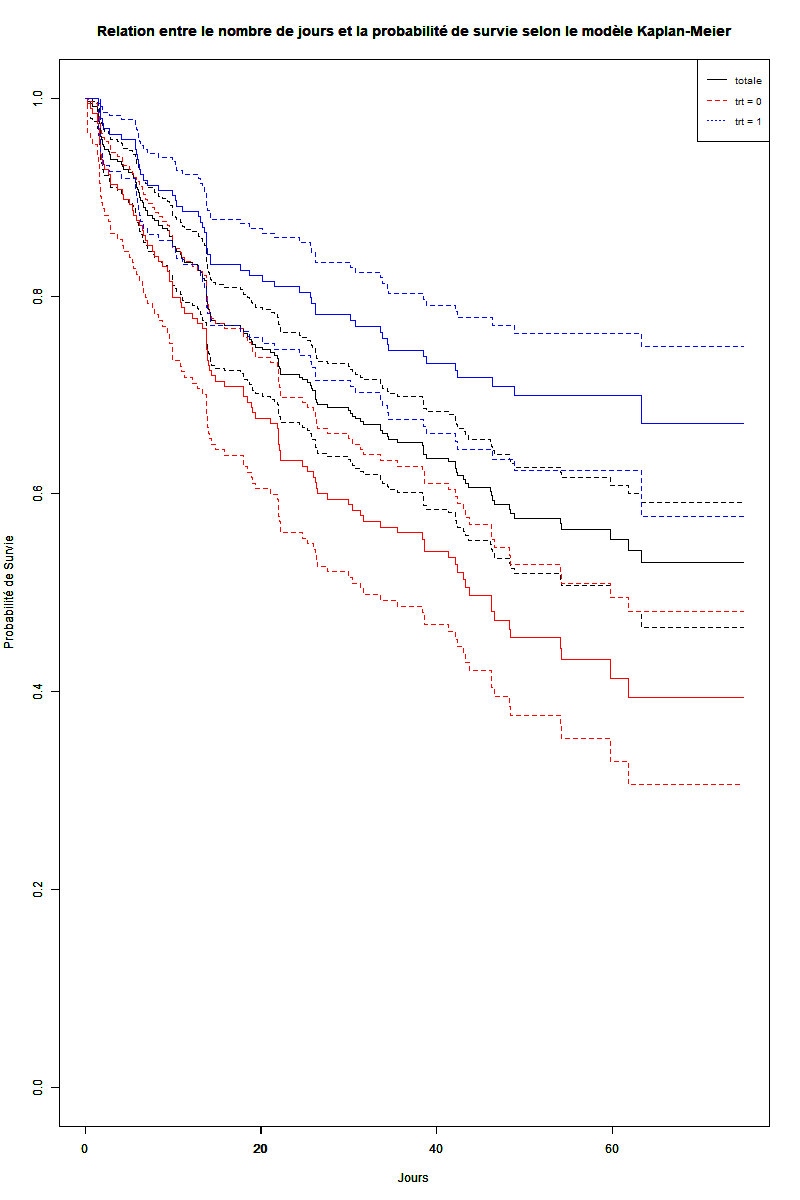
\includegraphics[width=0.6\textwidth]{1bc.png}
  \label{fig:mesh1}
\end{figure}

Les courbes, avec les bornes d'intervalles de confiance à $95 \%$, commencent à $1$ 
(c'est-à-dire, une probabilité de survie de $100 \%$) 
et diminue progressivement.
Par conséquent, il y a plus de risques de devenir aveugle au fil du temps.
On remarque aussi que les courbes ne sont pas lisses :
on ajoute information chaque fois qu'un événement se produit.
Le graphique montre aussi qu'il y a suffisamment de preuve statistique
pour dire que le traitement aide à retarder l'apparition de la cécité
parce que la courbe de survie du groupe traité est significativement
plus élevée que celle du groupe contrôle à la plupart des moments. ////

\end{CJK*}
\end{document}

\end{CJK*}
\end{document}